%++++++++++++++++++++++++++++++++++++++++
% Don't modify this section unless you know what you're doing!
\documentclass[letterpaper,12pt]{article}
\usepackage{tabularx} % extra features for tabular environment
\usepackage{amsmath}  % improve math presentation
\usepackage{graphicx} % takes care of graphic including machinery
\usepackage[margin=1in,letterpaper]{geometry} % decreases margins
\usepackage{cite} % takes care of citations
\usepackage[final]{hyperref} % adds hyper links inside the generated pdf file
\usepackage{float}
\hypersetup{
	colorlinks=true,       % false: boxed links; true: colored links
	linkcolor=blue,        % color of internal links
	citecolor=blue,        % color of links to bibliography
	filecolor=magenta,     % color of file links
	urlcolor=blue         
}
%++++++++++++++++++++++++++++++++++++++++
\numberwithin{equation}{section}

\begin{document}

\title{Machine Learning Homework1 Report}
\author{Diyang Gong, Xiaotong Li, and Yuxuan Liu \\
Student ID: 1635066,1634362,1632446}
\date{\today}
\maketitle


\begin{abstract}
In this group assignment, what we have is an assemble of training set and an assemble of test set. $k$-fold(in this case $k=10$) cross validation is used in this assignment to find the best value of lambda and report the loss on the test set. In addition, we prove that the regularization parameter $\lambda$ can solve the over-fit problem in 9-degree polynomial curve fitting.
\end{abstract}




\section{Theory}
\subsection{Cross Validation}

In the cross validation method, we need to categorize the training set into 2 groups by using $k$-fold function, which means divide the train data set into actual training set and validation set. Secondly, we try different $\lambda$ values, and calculate the coefficient $w$ for the polynomial, then leads to the square mean error for the training set points comparing with the corresponding points on the polynomial curve. After repeating $k$ times and making sure that every data in the train set only used once, we can find the optimal $\lambda$ for this degree's polynomial curve. The $k$ results from the folds can then be averaged to produce a single estimation\cite{mclachlan2005analyzing}.%在这里有个引用


\subsection{Polynomial Curve Fitting}
The meaning of polynomial curve fitting is that when we can get access to a bunch of data and try to build a model based on these data to predict how the values of data would be in specific conditions (ex.$y = f(x)$). By using polynomial curve fitting we can not only get the accurate-like value which is $y$ under certain $x$, we can also draw the trend of data. However, using higher degree of polynomial curve doesn't mean a better curve fitting, it might oscillate heavily and has over-fit problem. In this homework, we try to use degree 9 as our polynomial curve fitting degree.

%\begin{equation} \label{eq:aperp} % the label is used to reference the equation
%u(\lambda,T)=\frac{8\pi hc\lambda^{-5}}{e^{hc/\lambda kT}-1},
%\end{equation}
%where T is temperature in Kelvin, c is the speed of light, etc. Don't forget to
%explain what each variable means the first time that you introduce it.



\subsection{Regularization}
One technique that is often used to control the over-fit phenomenon is regularization, which involves adding a penalty term to the error function\cite{bishop2006pattern}
\begin{equation}\label{1.1}
E(w) = \frac{1}{2}\sum_{n=1}^{N}\left\{y(x_n,w)-t_n\right\}^2.
\end{equation}
%In order to discourage the coefficients from reaching large values. The simplest such penalty term takes the form of a sum of squares of all of the coefficients, leading to a modified error function of the form 
In order to overcome the curve over-fit the data points, the addition of a penalty item is necessary to prevent the occurrence of this phenomenon before the calculation of the error as Equation shown below.
\begin{equation}\label{1.2}
\widetilde{E}(w) = \frac{1}{2}\sum_{n=1}^{N}\left\{y(x_n,w)-t_n\right\}^2+\frac{\lambda}{2}{\left\|{w}\right\|}^2,
\end{equation}
where
\begin{equation}\label{1.3}
{\left\|{w}\right\|}^2=w^Tw=w_{0}^{2}+w_{1}^{2}+\cdots+w_{M}^{2}.
\end{equation}
and the coefficient $\lambda$ governs the relative importance of the regularization term compared with the sum-of-squares error term\cite{bishop2006pattern}.


\subsection{Overfit}
The curve fitting of the input training set matches well with the training set, yet matches bad with the validation set. The over-fit curve is made so strictly that any data (in this case validation set) which shows a little bit difference would not be recognized as part of the curve.




\section{Simulation Results and Analysis}

\subsection{$\lambda$}
Based on the theory of regularization, consider the $\lambda$ from large-scale to small-scale as shown in Fig.\ref{fig:large_scale} and Fig.\ref{fig:small_scale}. Firstly, we set the $\ln{\lambda}$ from -100 $\sim$ 0, and we can see from the Fig.\ref{fig:small_scale} that between the value of -10 $\sim$ 0, there is the nearly minimum value of $E_{MS}$, which is root-mean-square error. In the process of calculating the $E_{MS}$, we use the method called $k$-fold cross validation, which has been explained in the theory part. Then, we shrink our search range until find the optimal $\lambda$ as shown in Fig.\ref{fig:small_scale}. Finally, we choose the $\lambda=0.0408$ as the best selection and the $E_{MS}=0.29$. %(Err 关于lambda取值图片). 

\begin{figure}[H]
\vspace{-8.5cm}
 
\centering
      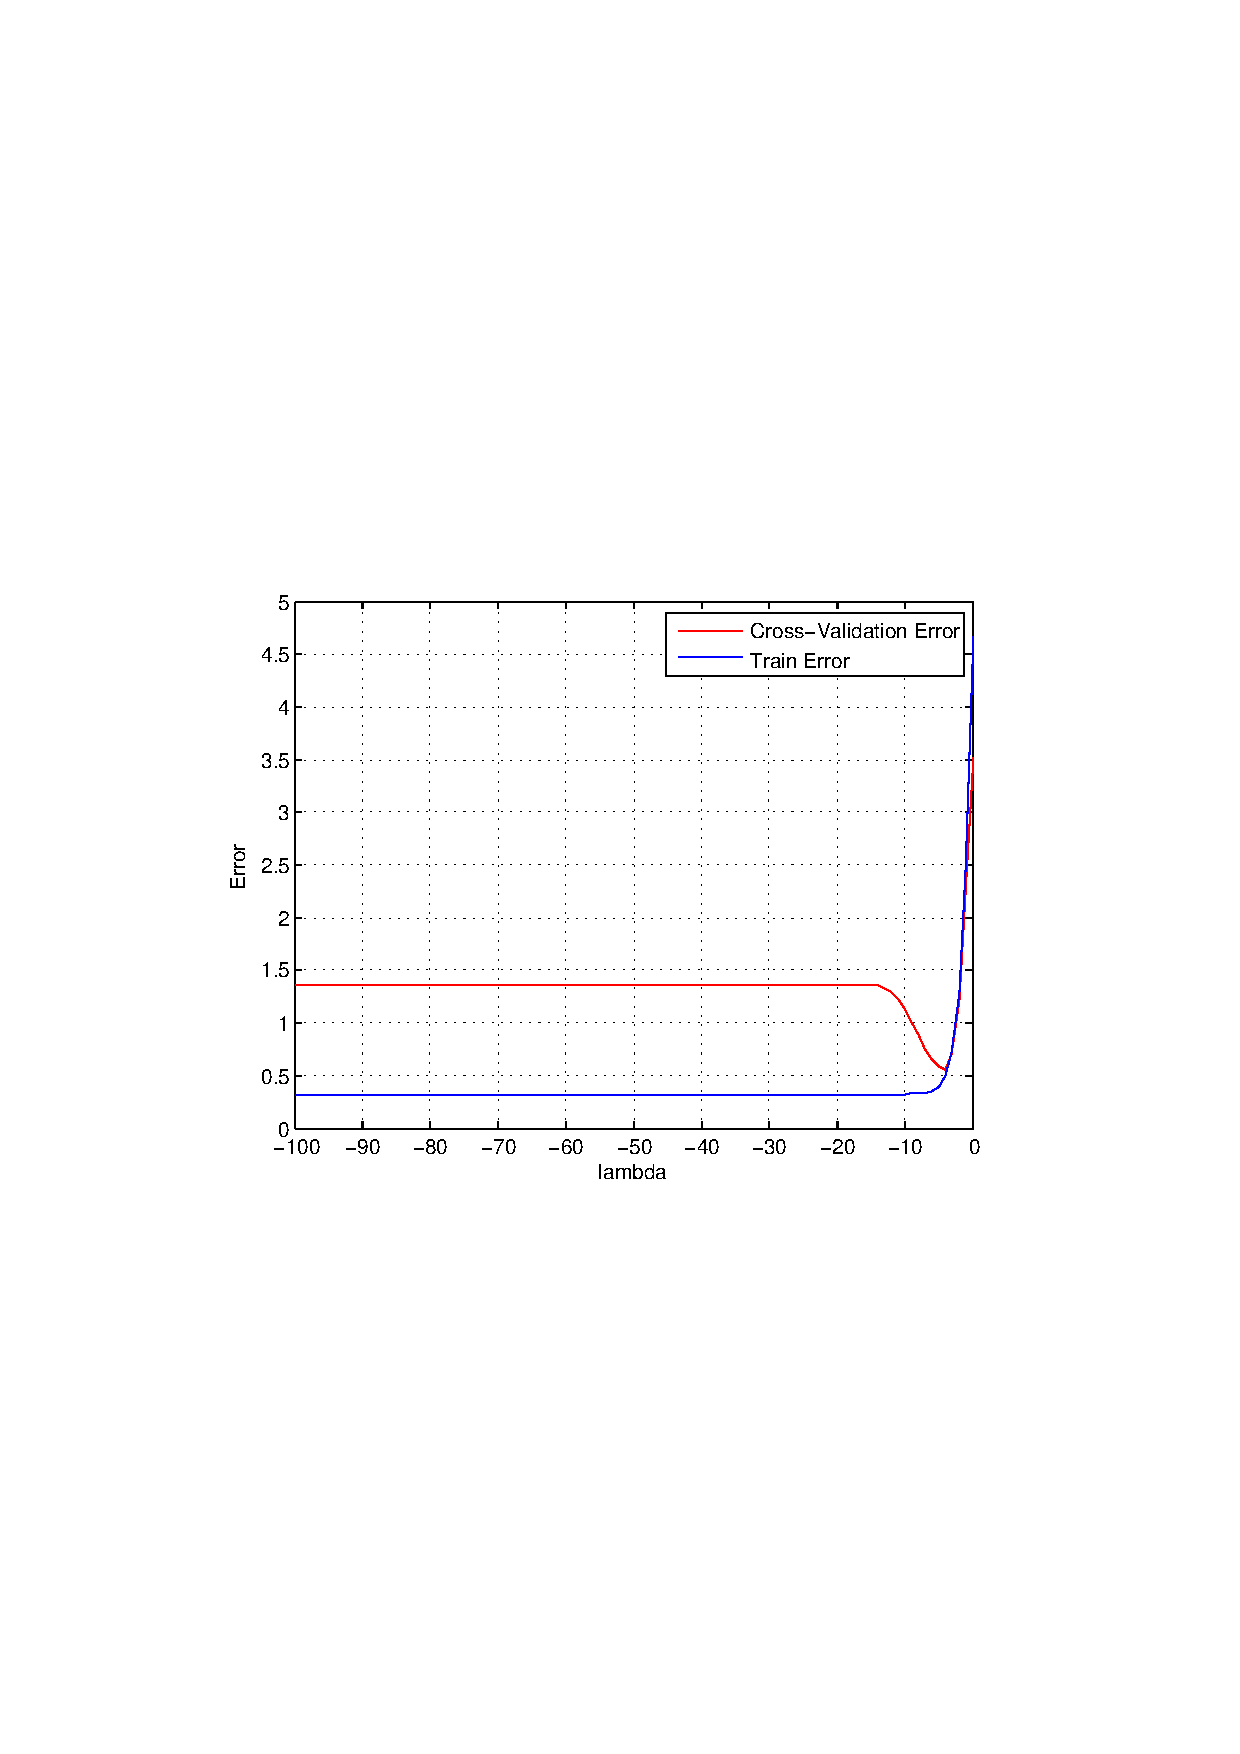
\includegraphics[scale=0.8]{-100-0}
% some figures do not need to be too wide
\vspace{-8.3cm}
\caption{\label{fig:large_scale} 
The relationship between large-scale $\lambda$ and error.}
       
\end{figure}




\begin{figure}[H]
\vspace{-8.5cm}
 
\centering
      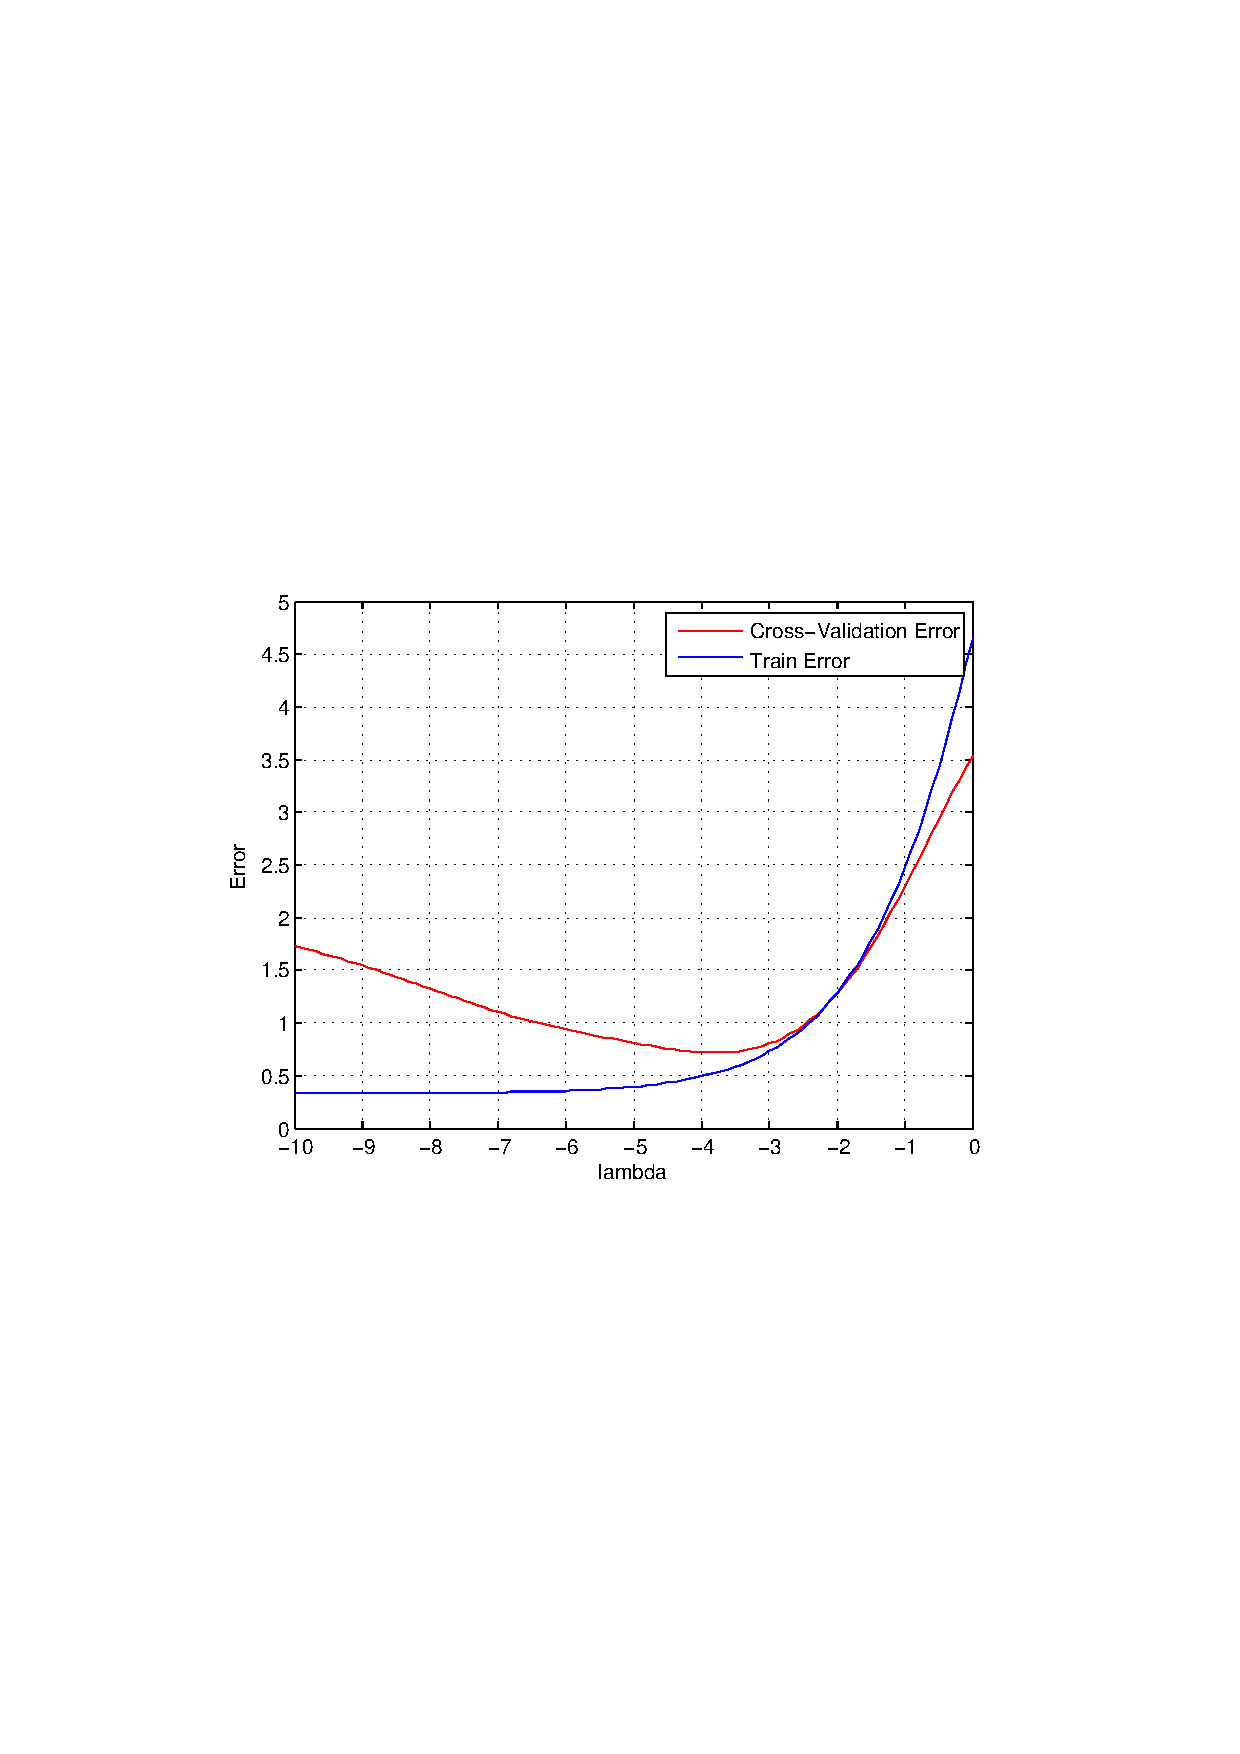
\includegraphics[scale=0.8]{-10-0}
% some figures do not need to be too wide
\vspace{-8.3cm}
\caption{\label{fig:small_scale} 
The relationship between small-scale $\lambda$ and error.}
       
\end{figure}


\subsection{$w^{*}$}
After setting the $\lambda$ value, we train the whole date set, then obtain the optimal combination of $w_{i}^{*} \left(i=0 \ldots 9 \right)$, which is shown below as Eq.\eqref{2.1}. So we can obtain the polynomial curve with the value of $w^{*}$, as shown in Fig.\ref{fig:curve_fitting}. The mean error of train data set is $E_{tr}=0.096$ based on Eq.\eqref{1.2}. In addition, for further prove of the correctness, we calculate the error of the test set and the mean error of test set is $E_{test}=0.112$. 
 \begin{equation}\label{2.1}
 \vspace{+2cm}
 w_{i}^{*}=\left\{
 \begin{array}{l}
w_{0}^{*}=3.858 \\
w_{1}^{*}=-0.534 \\
w_{2}^{*}=-0.244 \\
w_{3}^{*}=0.137 \\
w_{4}^{*}=-0.041 \\
w_{5}^{*}=0.017 \\
w_{6}^{*}=-0.004 \\
w_{7}^{*}=0.001 \\
w_{8}^{*}=-3.000\times10^{-5} \\
w_{9}^{*}=6.812\times10^{-7} \\
\end{array}
\right.
 \end{equation}

\begin{figure}[H]
\vspace{-5cm}
 
\centering
      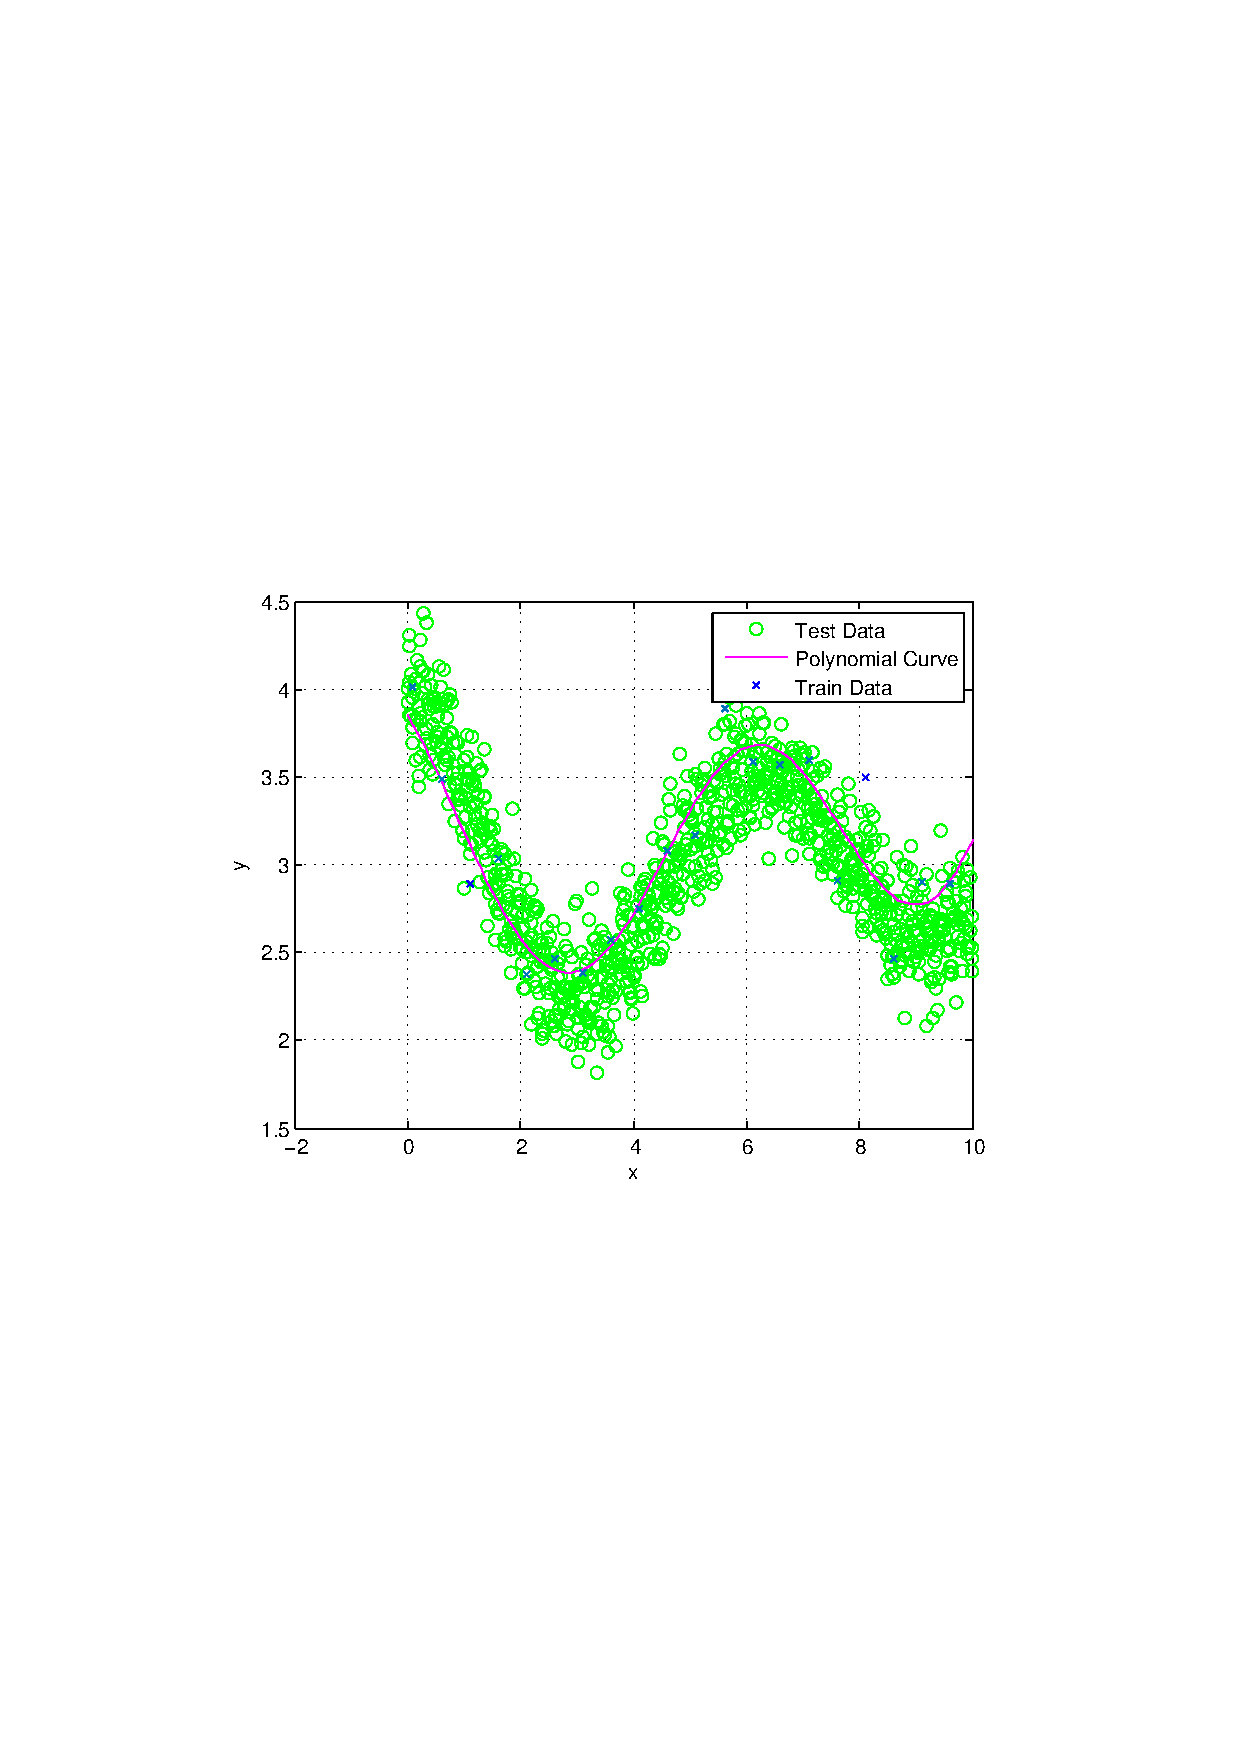
\includegraphics[scale=0.8]{1}
% some figures do not need to be too wide
\vspace{-8.3cm}
\caption{\label{fig:curve_fitting} 
Optimal curve fit with train data set and test data set.}
       
\end{figure}





\begin{figure}[htbp]
\vspace{-8.5cm}
 
\centering
      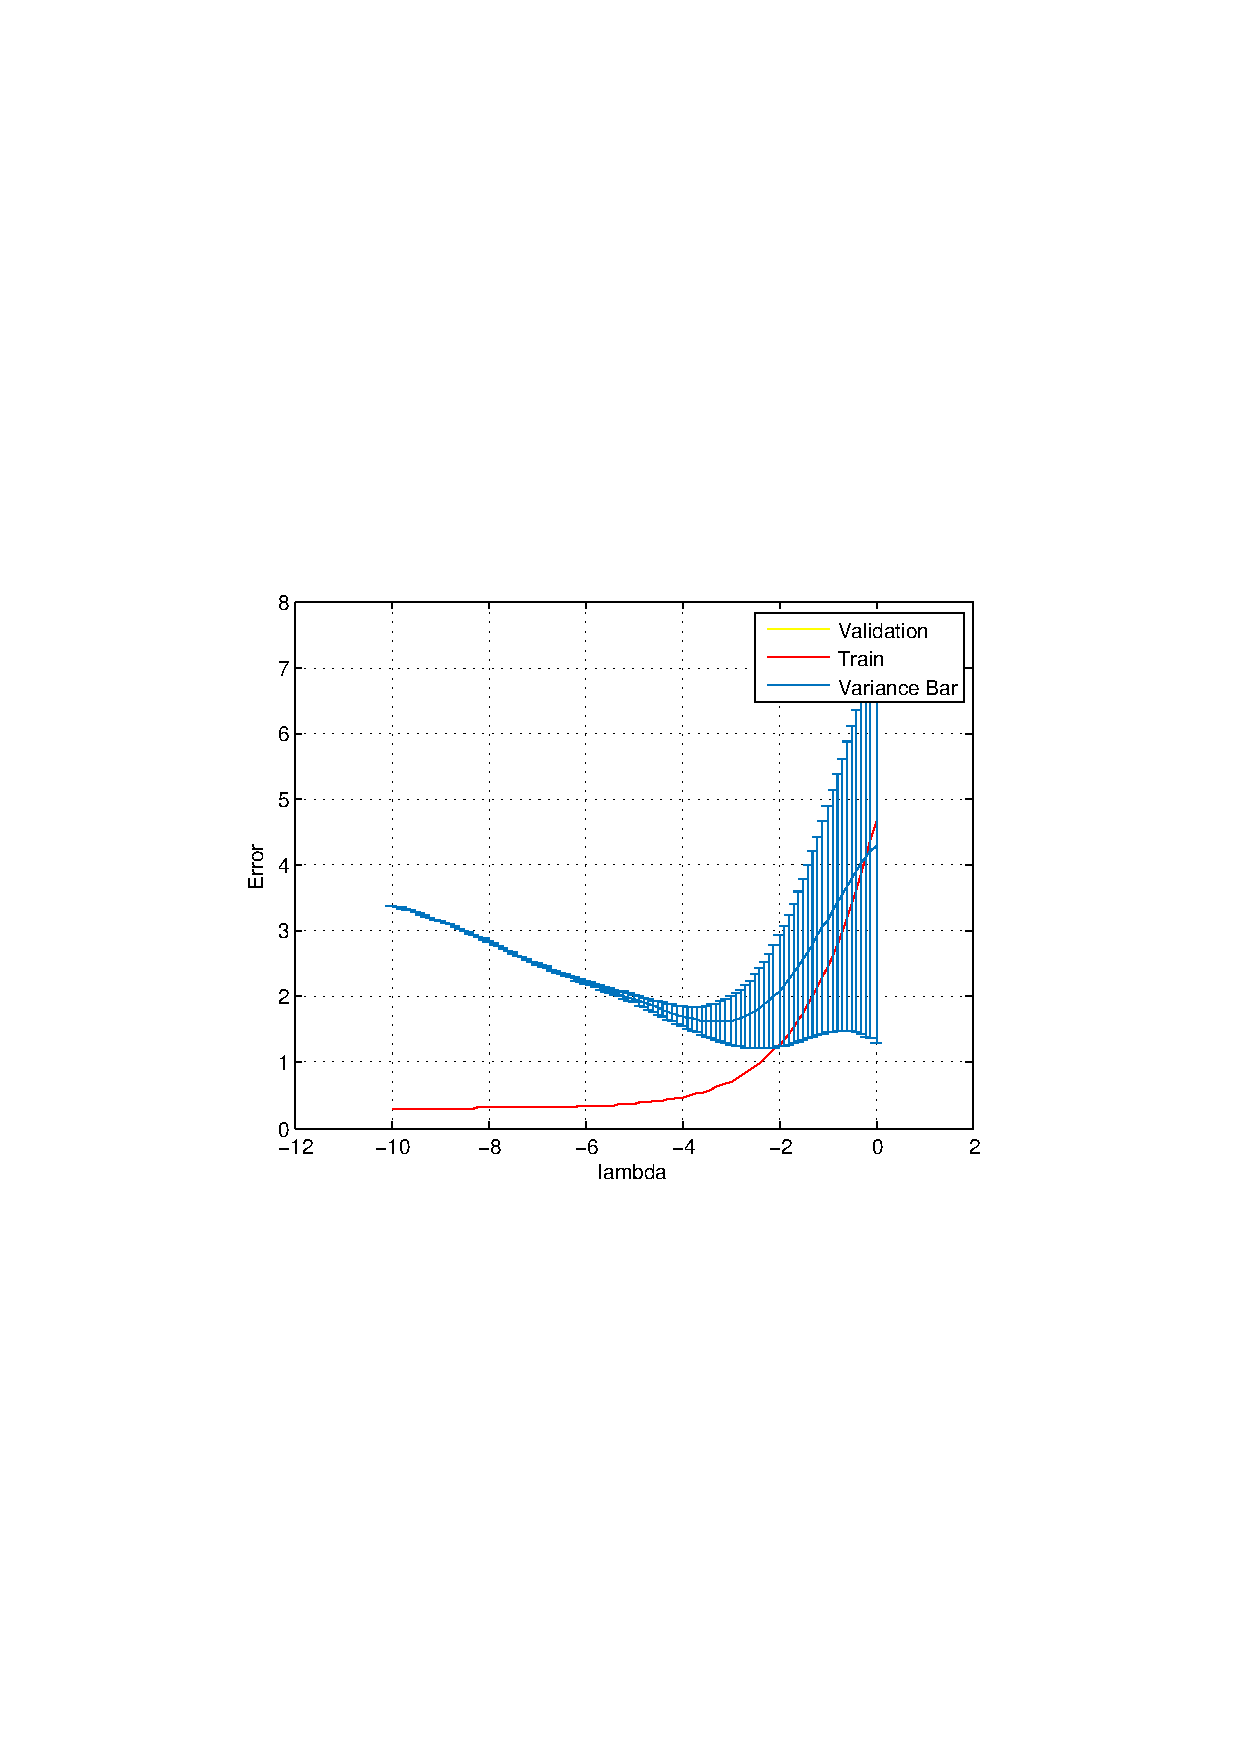
\includegraphics[scale=0.8]{2}
% some figures do not need to be too wide
\vspace{-8.3cm}
\caption{\label{fig:variance_bar} 
$\lambda$ effect on learning 9-degree polynomial curve fitting with 10-fold cross validation}
       
\end{figure}

\begin{figure}[H]
\vspace{-5cm}
 
\centering
      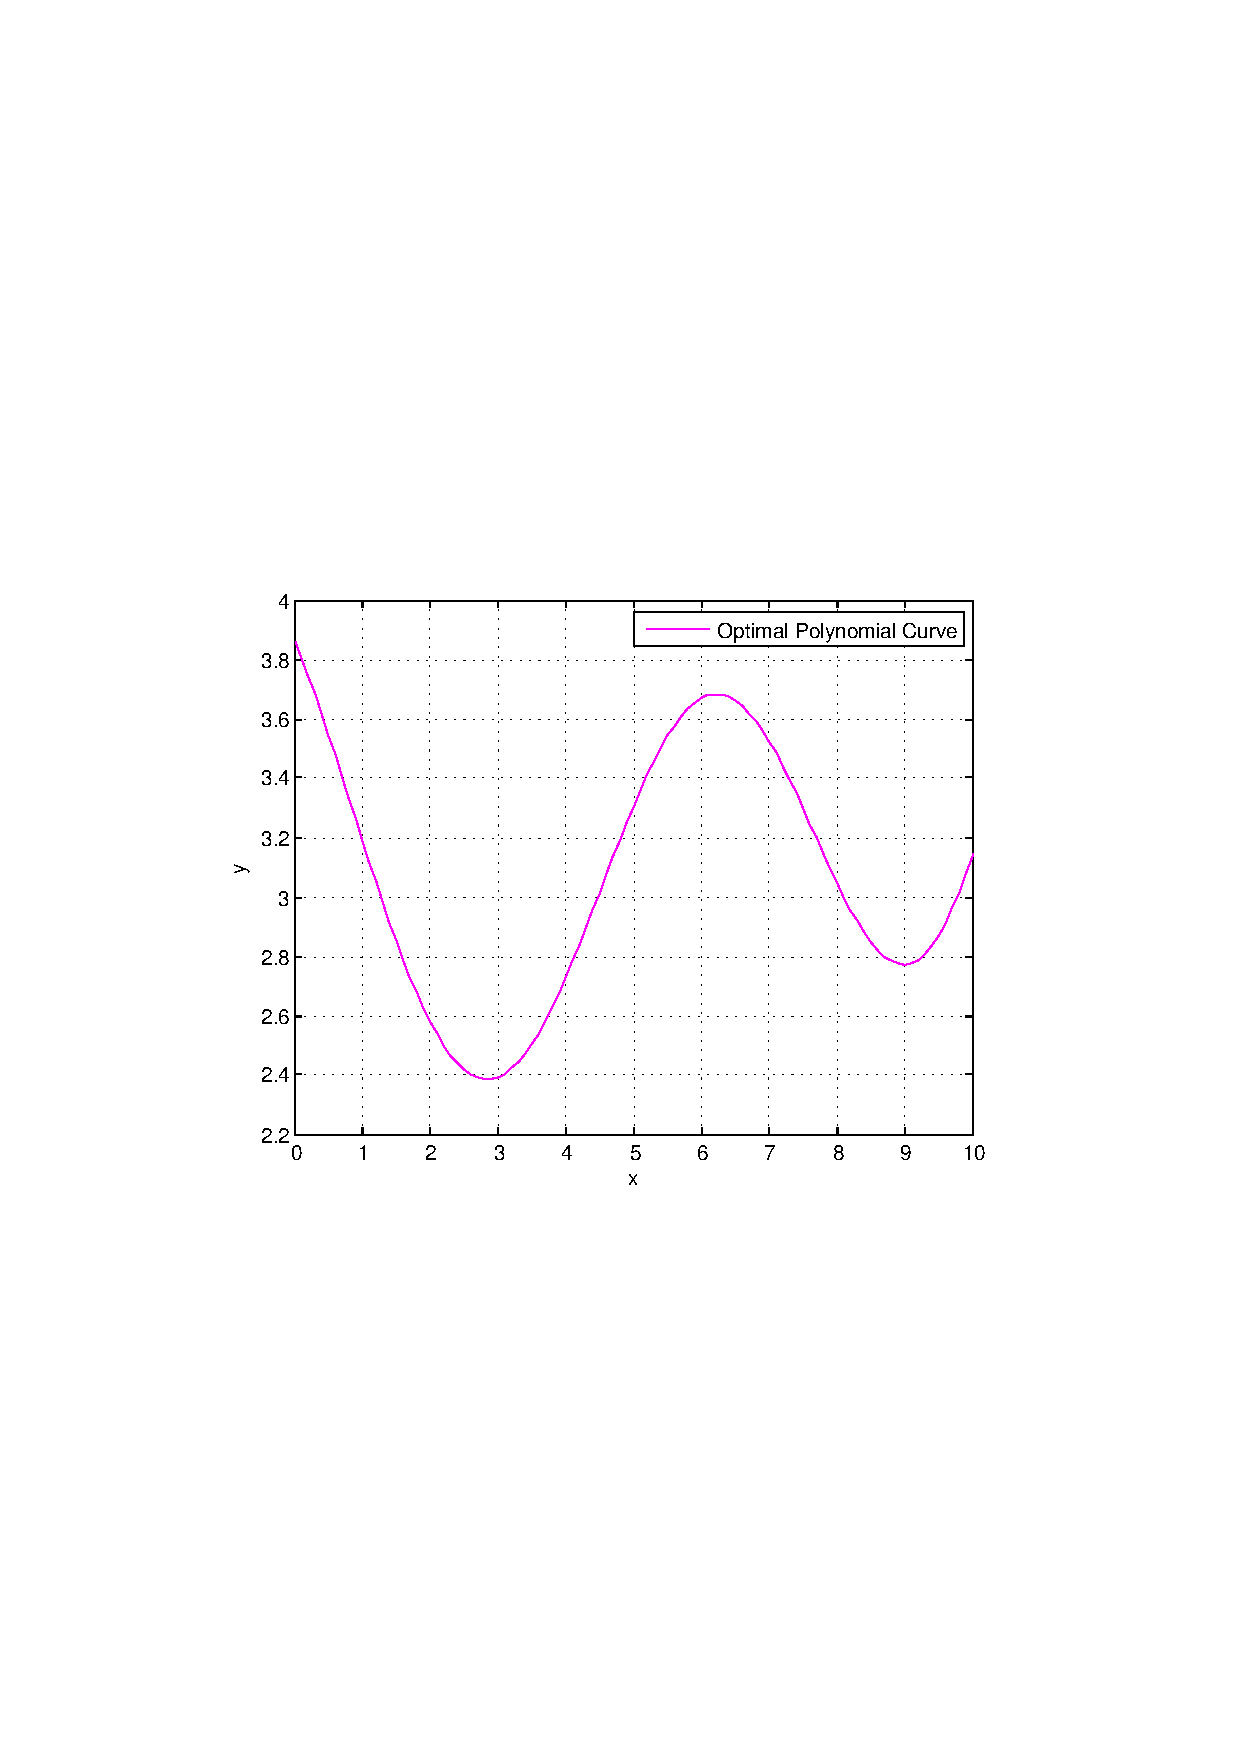
\includegraphics[scale=0.8]{3}
% some figures do not need to be too wide
\vspace{-8.3cm}
\caption{\label{fig:optimal curve} 
Optimal polynomial curve}
       
\end{figure}


\begin{figure}[H]
\vspace{-8.5cm}
 
\centering
      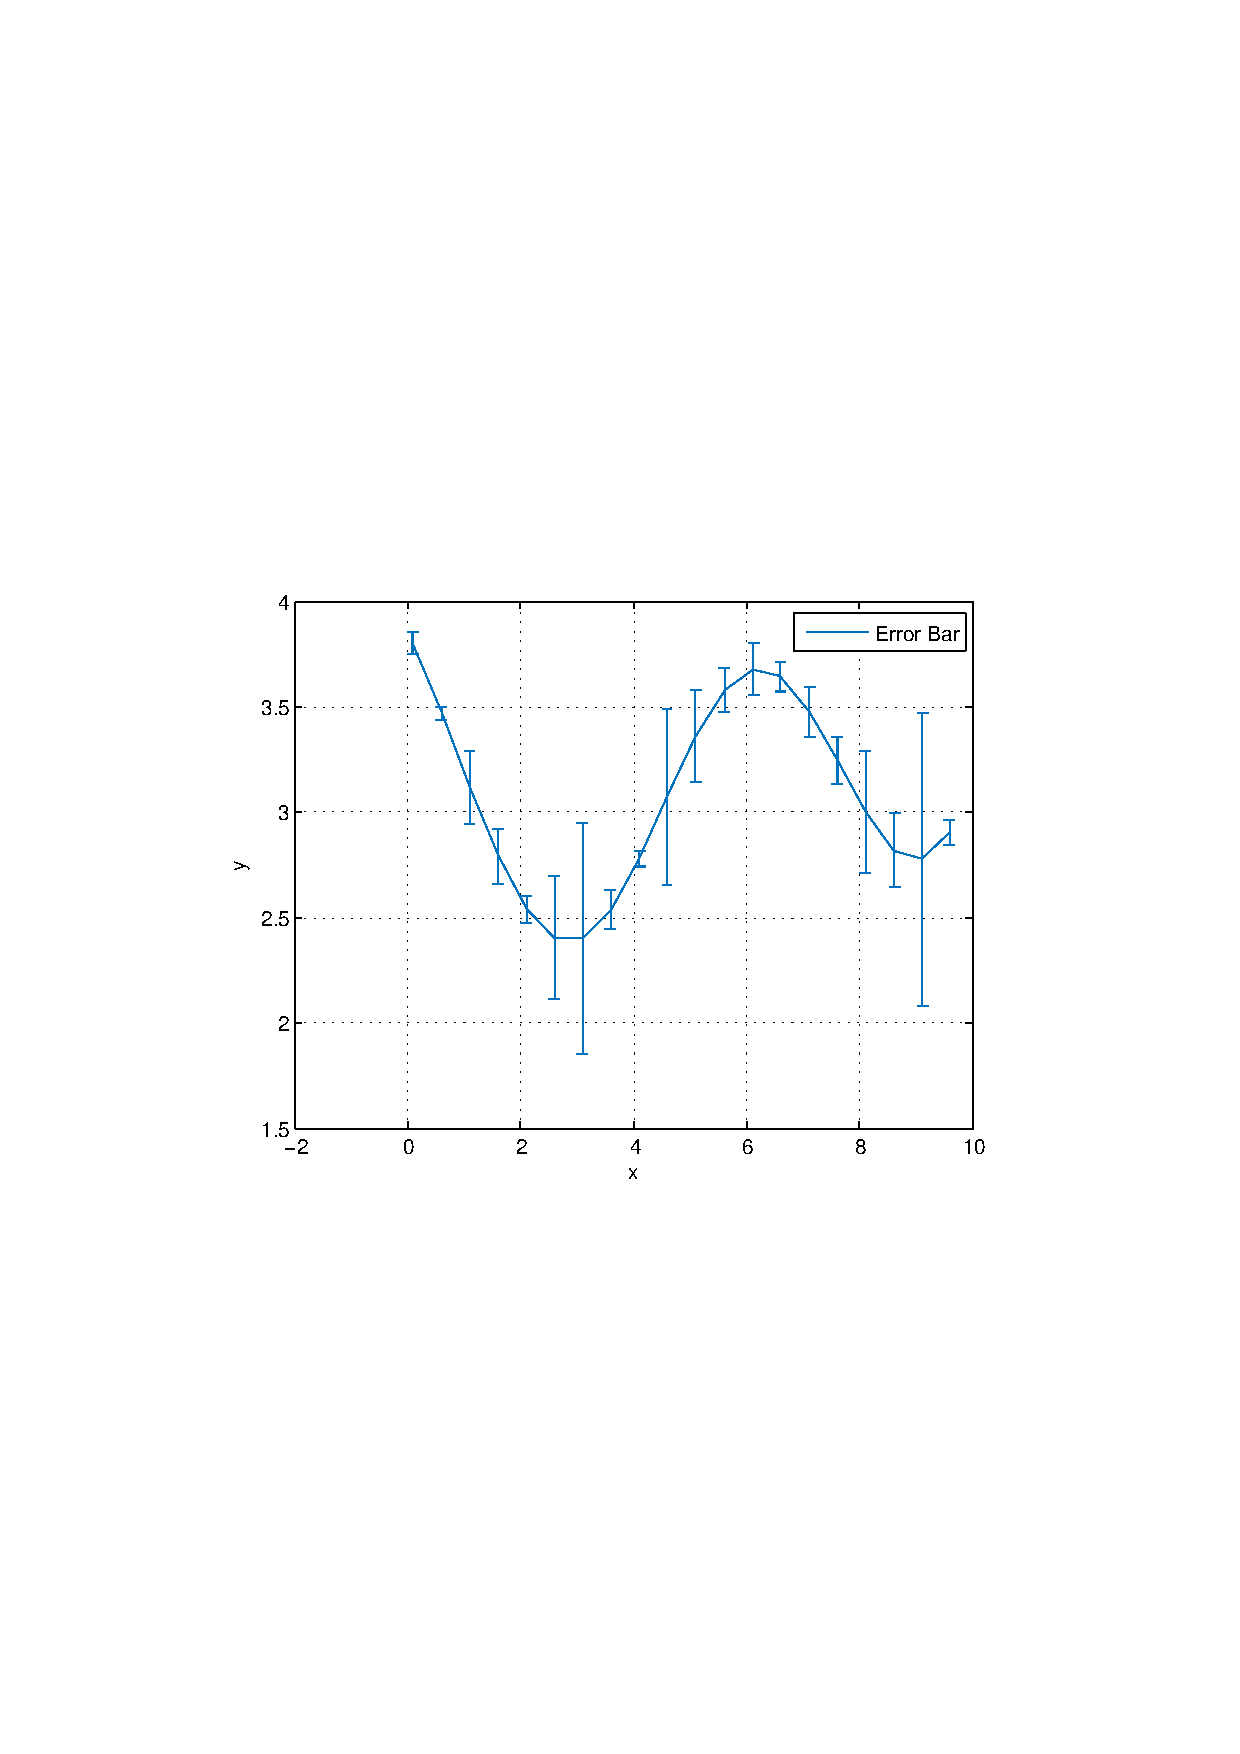
\includegraphics[scale=0.8]{4}
% some figures do not need to be too wide
\vspace{-8.3cm}
\caption{\label{fig:error_bar} 
$w$ effect on learning 9-degree polynomial curve fitting with 10-fold cross validation}
       
\end{figure}

\begin{figure}[H]
\vspace{-8.5cm}
 
\centering
      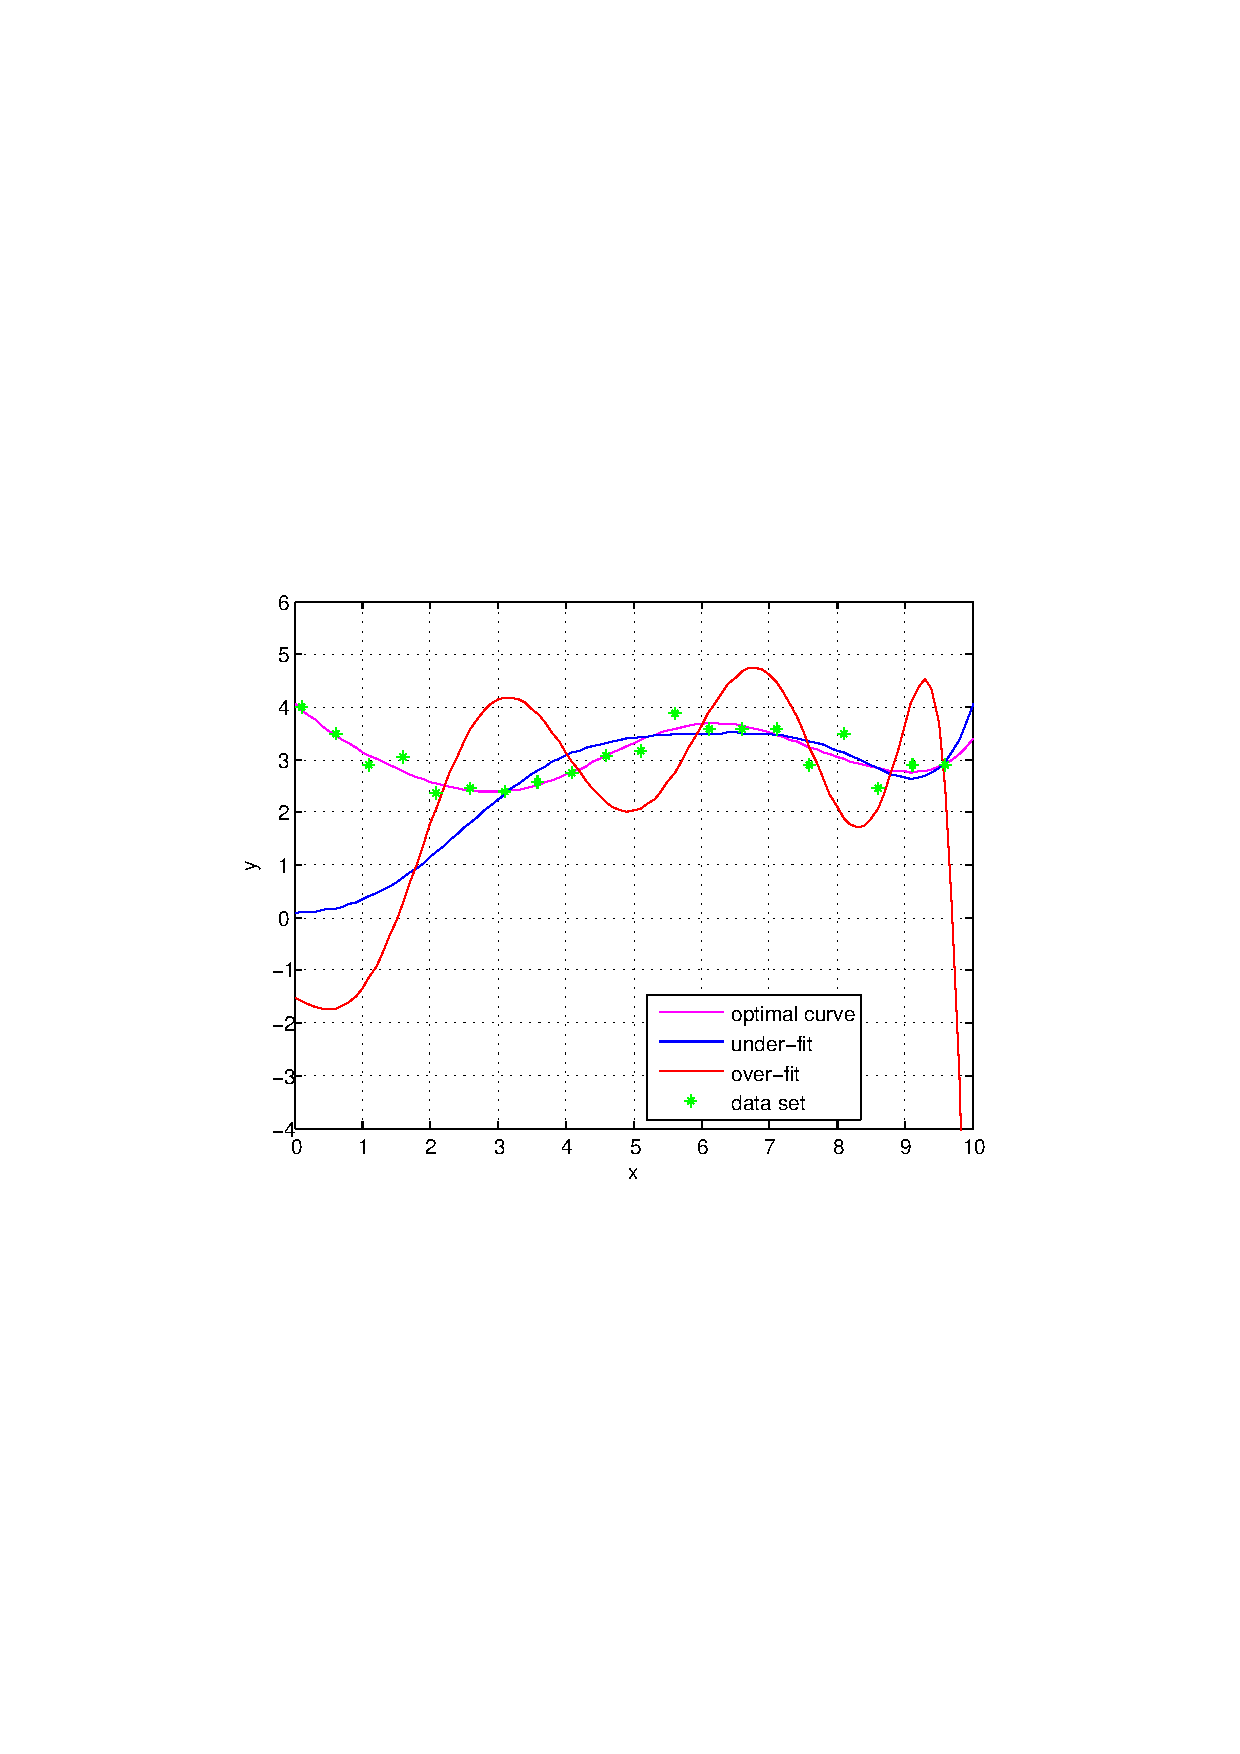
\includegraphics[scale=0.8]{untitled}
% some figures do not need to be too wide
\vspace{-8.3cm}
\caption{\label{fig:over_fit} 
$\lambda$ effect on learning 9-degree polynomial curve fitting with 10-fold cross validation}
\end{figure}

\section{Conclusions}
We find that the curve of $\lambda$-RMS(root-mean-square) is nearly a quadratic function. Thus, we get the optimal $\lambda$ by searching from the large-scale to the small-scale. We can see from the Fig.\ref{fig:curve_fitting} and Fig.\ref{fig:over_fit} $x-y$ that our polynomial curve fit both the whole data set and the test set very well. The value of error $E_{tr}$ and $E_{test}$ also prove it. Through this homework, we learn how to use $k$-fold cross validation and the normal equation with MATLAB, and use the regularization parameter $\lambda$ to overcome the over-fit or under-fit problem.


%++++++++++++++++++++++++++++++++++++++++
% References section will be created automatically 
% with inclusion of "thebibliography" environment
% as it shown below. See text starting with line
% \begin{thebibliography}{99}
% Note: with this approach it is YOUR responsibility to put them in order
% of appearance.

\begin{thebibliography}{99}

\bibitem{mclachlan2005analyzing}
McLachlan, Geoffrey and Do, Kim-Anh and Ambroise, Christophe, \textit{Analyzing microarray gene expression data},Vol.422,John Wiley \& Sons, New York, 2005.

\bibitem{bishop2006pattern}
Bishop, Christopher M,\textit{Pattern recognition and machine learning},Springer,2006
% "All-optical microwave frequency standard: a proposal,"
%IEEE Trans.\ Instrum.\ Meas.\ \textbf{42}, 640 (1993).

%\bibitem{Wiki} \emph{Expected value},  available at
%\texttt{http://en.wikipedia.org/wiki/Expected\_value}.


\end{thebibliography}


\end{document}
